\documentclass[a4paper, 12pt]{article}
\usepackage[spanish]{babel}
\usepackage[hmargin=2cm,vmargin=2.5cm]{geometry}
\usepackage{enumerate}
\usepackage{makecell}
\usepackage{graphicx}
\usepackage{hyperref}
\usepackage{amsmath}
\usepackage[backend=biber,style=apa, url=true, sortcites]{biblatex}
\usepackage[table]{xcolor}
\usepackage{minted}
\usepackage{graphicx}
\usepackage{fancyhdr}  % Agrega el paquete fancyhdr
\usepackage{subcaption}

\addbibresource{references.bib}
\hypersetup{
	colorlinks,
	citecolor=black,
	filecolor=black,
	linkcolor=black,
	urlcolor=black
}

\setlength{\arrayrulewidth}{0.4mm}

\newcommand{\HRule}{\rule{\linewidth}{0.5mm}}

\begin{document}
	\begin{titlepage}
		\begin{center}
			% logo
			
\includegraphics[width=0.5\textwidth]{figures/logoUAH.png}~\\[2cm]
			
			\textsc{\Large \\Sistemas de Control Inteligente}\\[2cm]
			
			\HRule \\[0.4cm]
			{\LARGE \bfseries Práctica 0. \\ Introducción a Matlab \\[0.4cm]}
			\HRule \\[3cm]
			
			\large\textbf{Jorge Revenga Martín de Vidales}\\
			\large\textbf{Ángel Salgado Aldao}\\
			\large\textbf{}\\ Grado en Ingeniería Informática \\ Universidad de Alcalá
			
			\vfill
			
			{\large \today}
		\end{center}
	\end{titlepage}
	
	% Configura los encabezados y pies de página
	\pagestyle{fancy}
	\fancyhf{} % Limpia todos los encabezados y pies de página actuales
	% Encabezado
	\fancyhead[RO,LE]{\textit{Sistemas de Control Inteligente}}
	\fancyhead[LO,RE]{\textit{Ejercicios de Introducción a Matlab}}  % Título del documento
	% Pie de página
	\fancyfoot[LO,RE]{\textit{Universidad de Alcalá}}
	\fancyfoot[RO,LE]{\thepage}  % Número de página en la esquina inferior derecha
	\newpage
	
	\thispagestyle{plain}
	\tableofcontents
	\newpage
    
    \part{}
	
	\section{Ejercicio 1. Matrices y vectores.}
	
	\subsection{Código}
	\inputminted[fontsize=\scriptsize, linenos, breaklines=true, xleftmargin=0.75cm, frame=lines]{matlab}{code/parte1/Ejercicio1.m}
	\subsection{Ejecución}
	\begin{figure}[htp!]
		\centering
		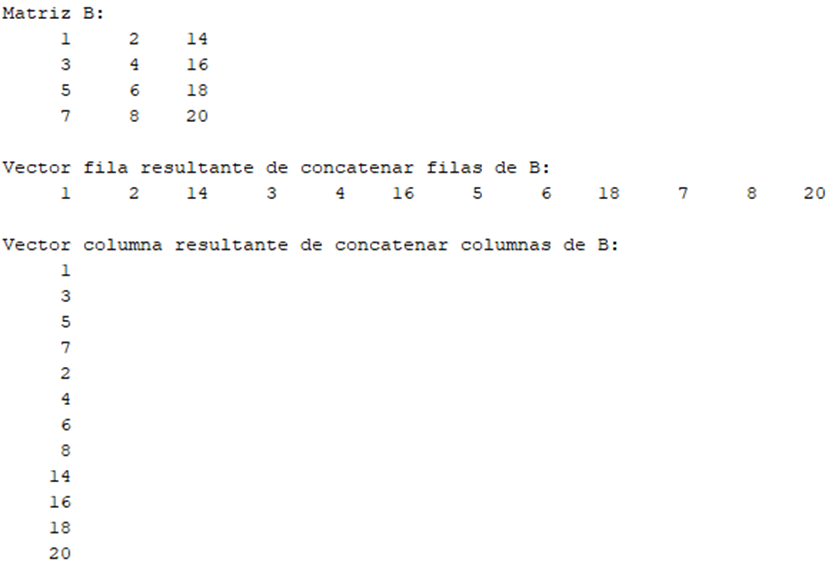
\includegraphics[width=0.7\textwidth]{figures/ejc1.png}
		\caption{Ejecución ejercicio 1.}
	\end{figure}
	
	\section{Ejercicio 2. Matrices y vectores.}
	
	\subsection{Código}
	\inputminted[fontsize=\scriptsize, linenos, breaklines=true, xleftmargin=0.75cm, frame=lines]{matlab}{code/parte1/Ejercicio2.m}
	\subsection{Ejecución}
	\begin{figure}[htp!]
		\centering
		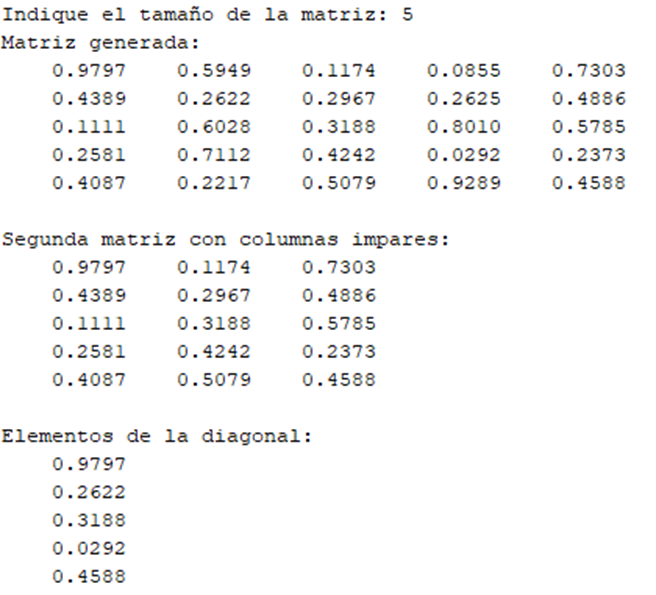
\includegraphics[width=0.6\textwidth]{figures/ejc2.png}
		\caption{Ejecución ejercicio 2.}
	\end{figure}
	\begin{figure}[htp!]
		\centering
		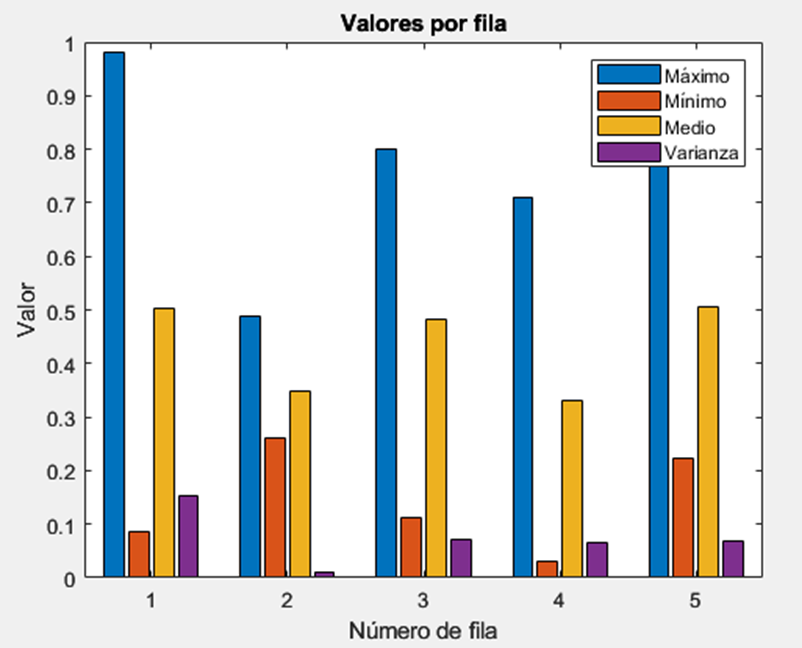
\includegraphics[width=0.6\textwidth]{figures/graf1.png}
		\caption{Gráfico ejecución ejercicio 2.}
	\end{figure}
	
	\section{Ejercicio 3. Matrices y vectores.}
	
	\subsection{Código}
	\subsection*{IntroducirMatriz.m}
	\inputminted[fontsize=\scriptsize, linenos, breaklines=true, xleftmargin=0.75cm, frame=lines]{matlab}{code/parte1/IntroducirMatriz.m}
	\inputminted[fontsize=\scriptsize, linenos, breaklines=true, xleftmargin=0.75cm, frame=lines]{matlab}{code/parte1/Ejercicio3.m}
	\newpage
        \subsection{Ejecución}
	\begin{figure}[ht]
		\begin{subfigure}{0.49\textwidth}
			\centering
			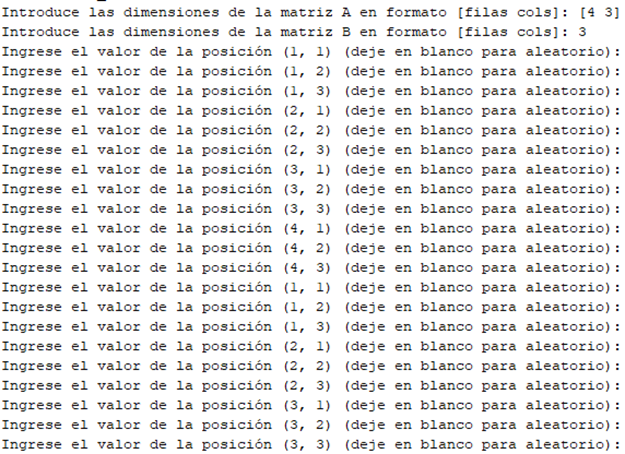
\includegraphics[width=\textwidth]{figures/ejc3.1.png}
			\label{grafica5.1}
		\end{subfigure}
		\begin{subfigure}{0.49\textwidth}
			\centering
			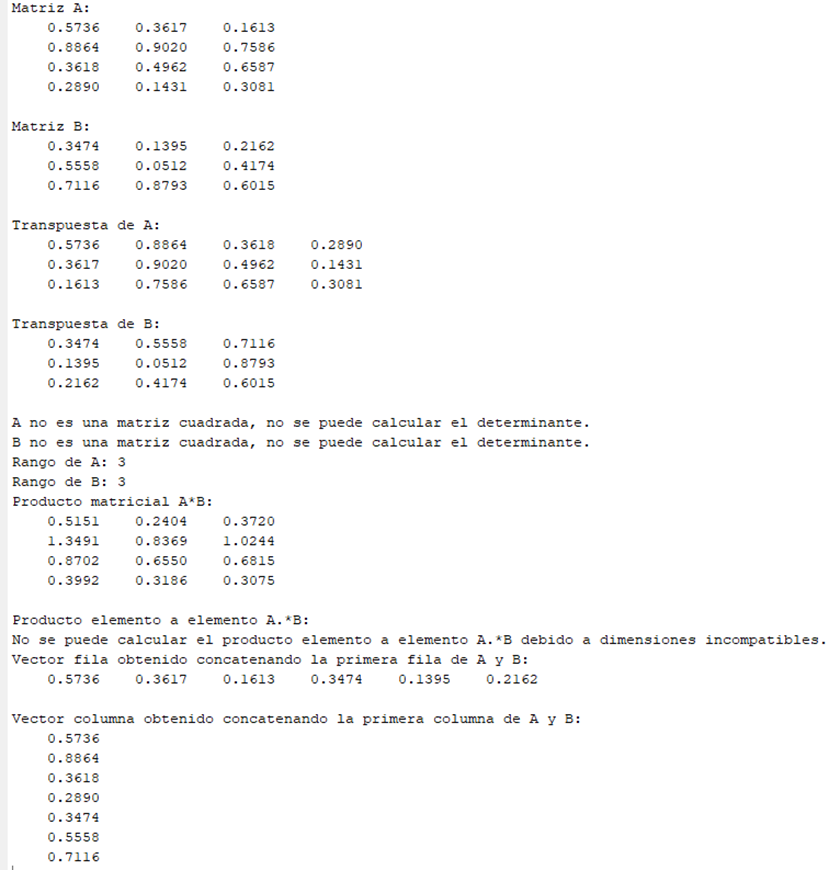
\includegraphics[width=\textwidth]{figures/ejc3.2.png}
			\label{grafica5.2}
		\end{subfigure}
		\caption{Ejecución ejercicio 3.}
		\label{ejec3}
	\end{figure}
	\newpage
 
	\section{Ejercicio 4. Tiempo de cómputo y representación gráfica.}
	
	\subsection{Código}
	\inputminted[fontsize=\scriptsize, linenos, breaklines=true, xleftmargin=0.75cm, frame=lines]{matlab}{code/parte1/Ejercicio4.m}
	\subsection{Ejecución}
	\begin{figure}[htp!]
		\centering
		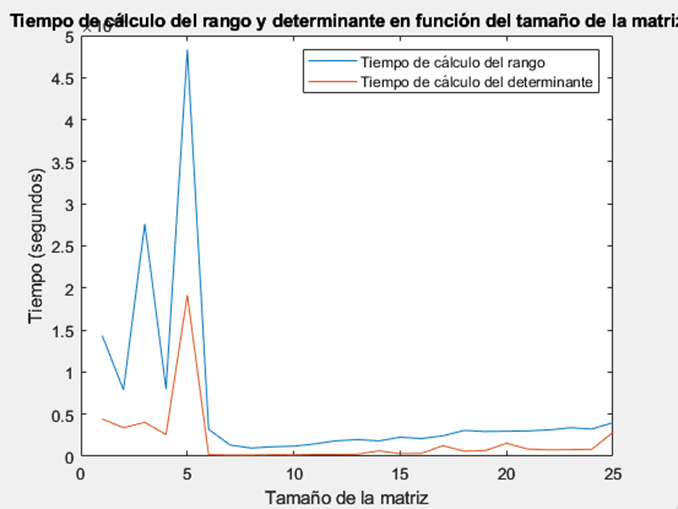
\includegraphics[width=0.6\textwidth]{figures/graf4.png}
		\caption{Gráfico ejecución ejercicio 4.}
	\end{figure}
	
	\section{Ejercicio 5. Representación gráfica en 3D.}
	
	\subsection{Código}
	\inputminted[fontsize=\scriptsize, linenos, breaklines=true, xleftmargin=0.75cm, frame=lines]{matlab}{code/parte1/Ejercicio5.m}
	\newpage
        \subsection{Ejecución}
	\begin{figure}[ht]
		\begin{subfigure}{0.49\textwidth}
			\centering
			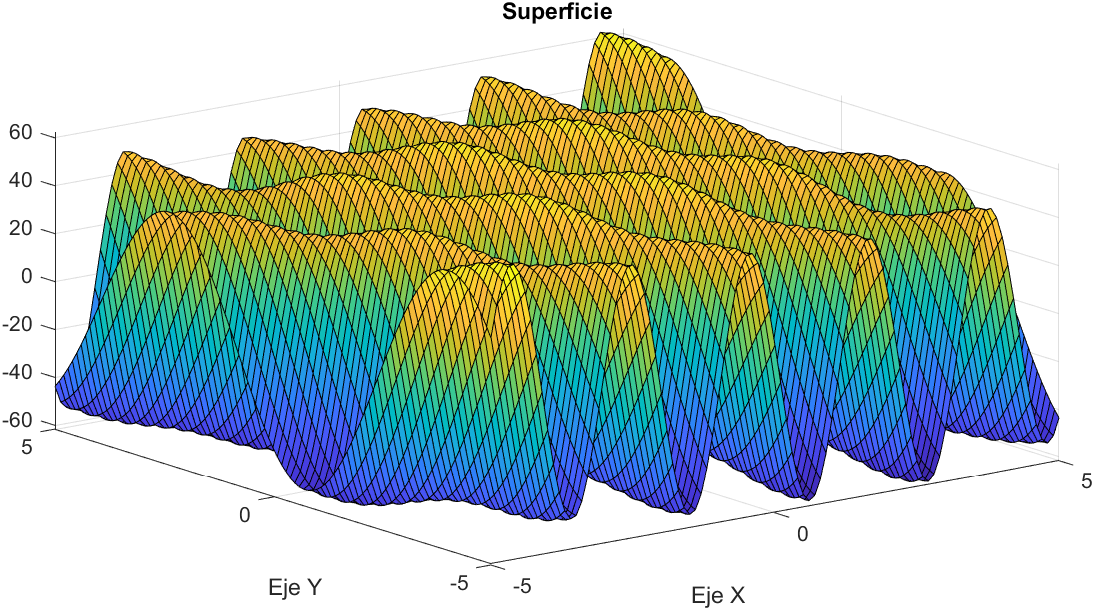
\includegraphics[width=\textwidth]{figures/graf5.1.png}
			\caption{Gráfico de superficie.}
			\label{grafica5.1}
		\end{subfigure}
		\begin{subfigure}{0.49\textwidth}
			\centering
			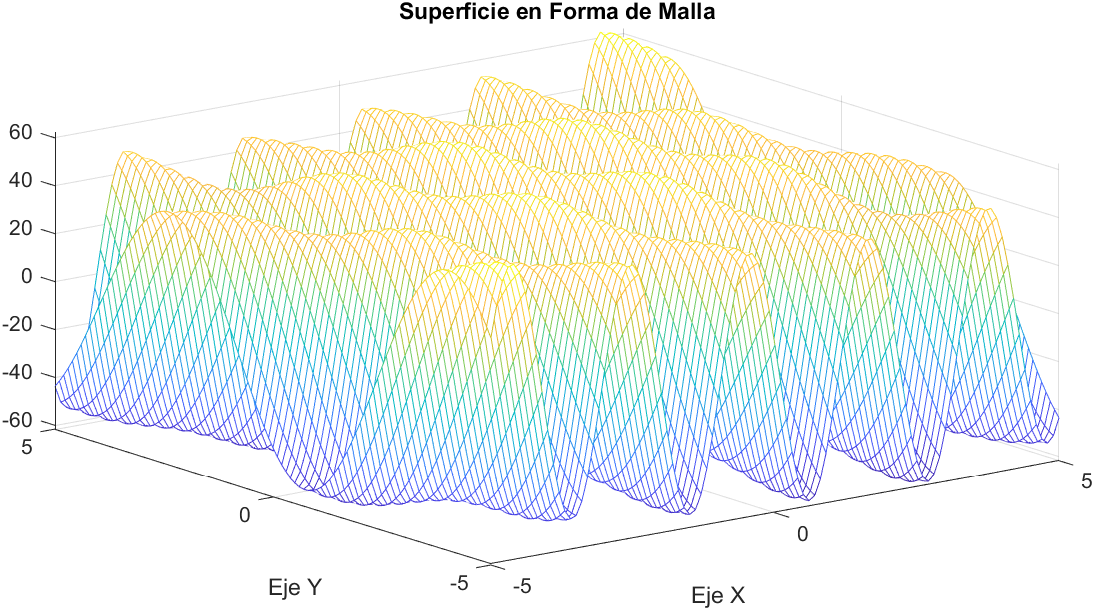
\includegraphics[width=\textwidth]{figures/graf5.2.png}
			\caption{Gráfico de superficie en forma de malla.}
			\label{grafica5.2}
		\end{subfigure}
		\begin{subfigure}{0.49\textwidth}
			\centering
			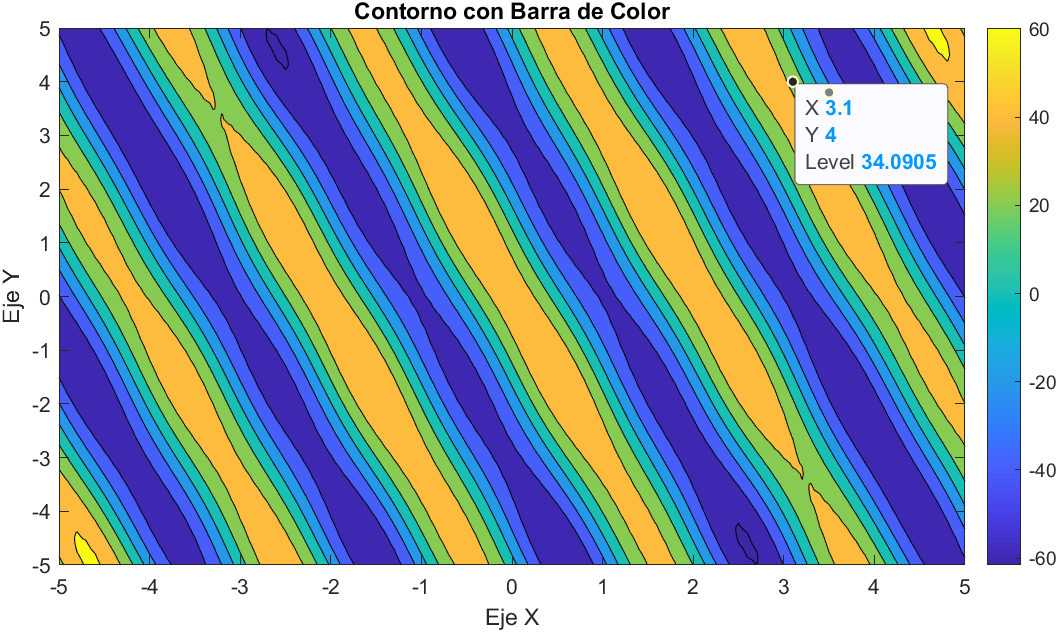
\includegraphics[width=\textwidth]{figures/graf5.3.png}
			\caption{Gráfico de contorno con barra de color.}
			\label{grafica5.3}
		\end{subfigure}
		\caption{Gráficos ejecución ejercicio 5.}
		\label{graficos5}
	\end{figure}

        \newpage
	\section{Ejercicio 6. Sistemas lineales.}
	
	\subsection{Código}
	\inputminted[fontsize=\scriptsize, linenos, breaklines=true, xleftmargin=0.75cm, frame=lines]{matlab}{code/parte1/Ejercicio6.m}
	\subsection{Ejecución}
	\begin{figure}[htp!]
		\centering
		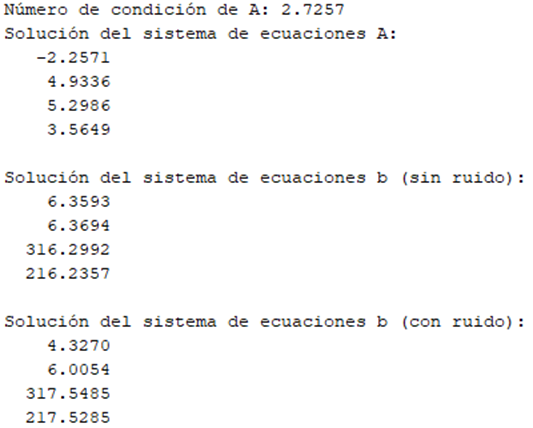
\includegraphics[width=0.6\textwidth]{figures/ejc6.png}
		\caption{Gráfico ejecución ejercicio 6.}
	\end{figure}
	
	\section{Ejercicio 7. Polinomios.}
	
	\subsection{Código}
	\subsection*{raices.m}
	\inputminted[fontsize=\scriptsize, linenos, breaklines=true, xleftmargin=0.75cm, frame=lines]{matlab}{code/parte1/raices.m}
	\inputminted[fontsize=\scriptsize, linenos, breaklines=true, xleftmargin=0.75cm, frame=lines]{matlab}{code/parte1/Ejercicio7.m}
	\newpage
        \subsection{Ejecución}
	\begin{figure}[ht]
		\centering
		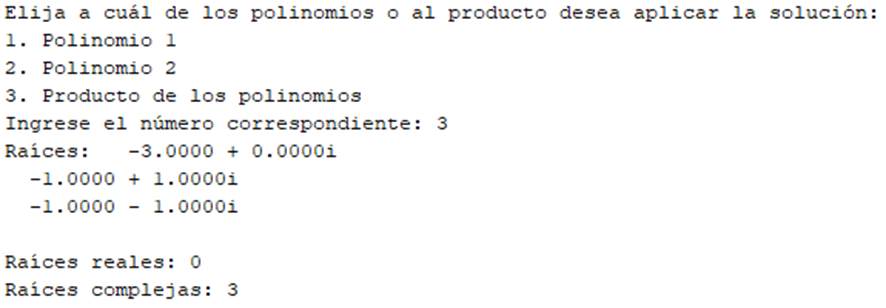
\includegraphics[width=0.6\textwidth]{figures/ejc7.png}
		\caption{Ejecución ejercicio 7.}
		\label{ejec7}
	\end{figure}
	\begin{figure}[ht]
		\centering
		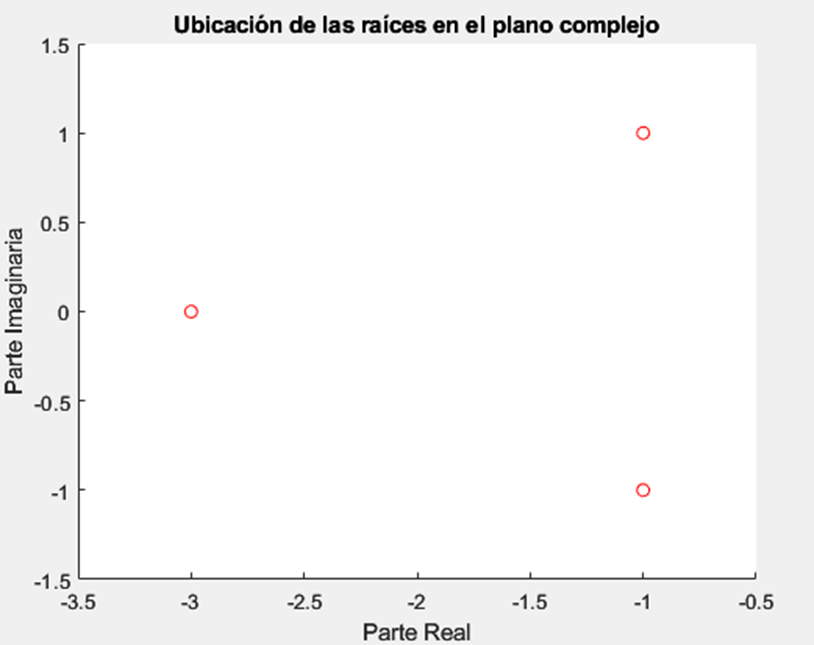
\includegraphics[width=0.5\textwidth]{figures/graf7.png}
		\caption{Gráfico ejecución ejercicio 7.}
		\label{grafica7}
	\end{figure}

    \newpage
    \part{}
    
    \section{Ejercicio 1. Transformadas de señales.}
    \subsection{}
	\paragraph{Obtenga la transformada z de la siguiente función:f(k) = 2 + 5k + $k^{2}$. Represente gráficamente las señales original y transformada.}
    \subsubsection*{Código}
	\inputminted[fontsize=\scriptsize, linenos, breaklines=true, xleftmargin=0.75cm, frame=lines]{matlab}{code/parte2/Ej1p1.m}

    \newpage
	\subsubsection*{Ejecución}
    \begin{figure}[ht]
		\begin{subfigure}{0.49\textwidth}
			\centering
			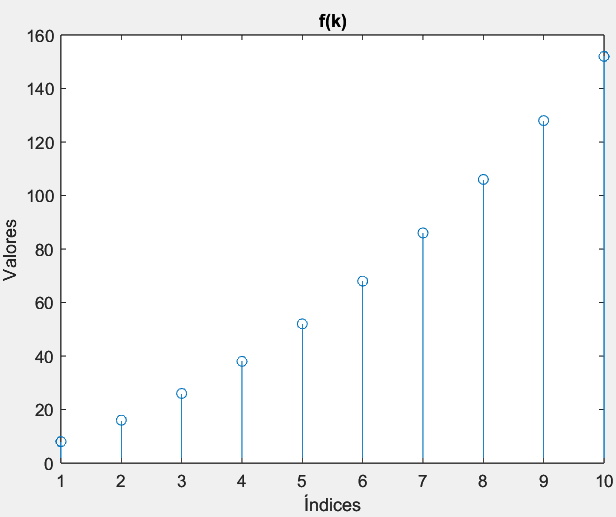
\includegraphics[width=1\textwidth]{figures/Parte2Ej1p1f1.png}
		\end{subfigure}
		\begin{subfigure}{0.49\textwidth}
			\centering
			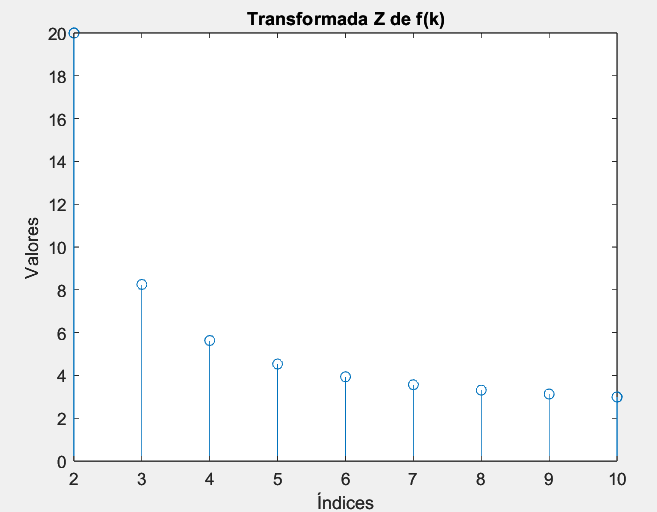
\includegraphics[width=1\textwidth]{figures/Parte2Ej1p1f2.png}
		\end{subfigure}
    \caption{Ejecución ejercicio 1.1.}
	\end{figure}

    \subsection{}
    \paragraph{Obtenga la transformada $z$ de la siguiente función: $f(k) = \sin(k) \cdot e^{-ak}$. Represente gráficamente, de nuevo, las señales original y transformada.}
    \subsubsection*{Código}
	\inputminted[fontsize=\scriptsize, linenos, breaklines=true, xleftmargin=0.75cm, frame=lines]{matlab}{code/parte2/Ej1p2.m}

	\subsubsection*{Ejecución}
    
    \begin{figure}[htp!]
        \centering
        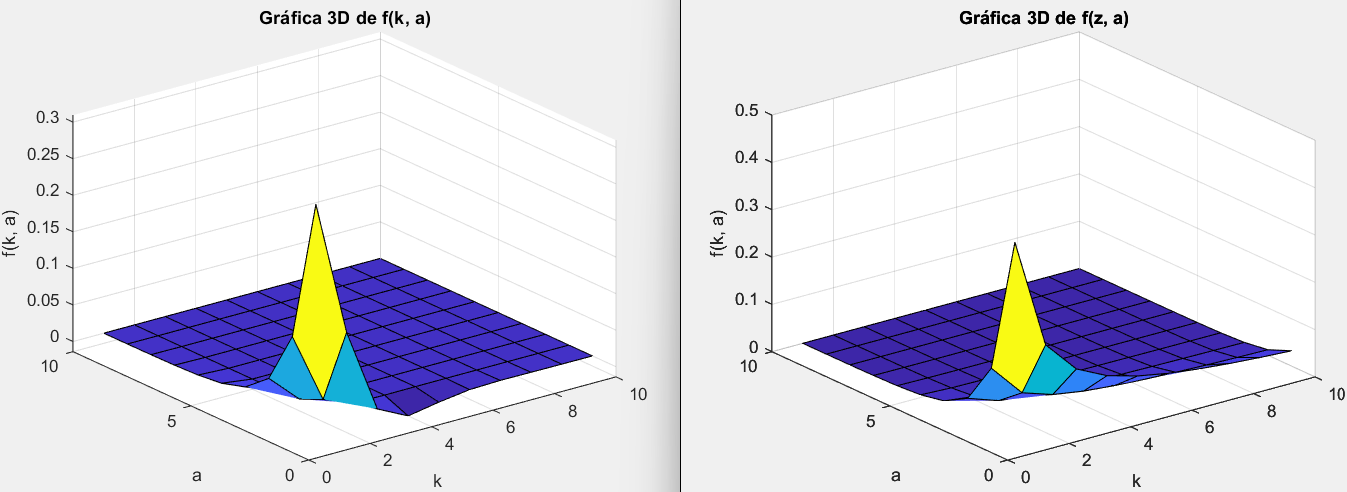
\includegraphics[width=1\textwidth]{figures/Parte2Ej1p2f1.png}
        \caption{Ejecución 1 ejercicio 1.2.}
    \end{figure}
        
    \begin{figure}[htp!]
        \centering
        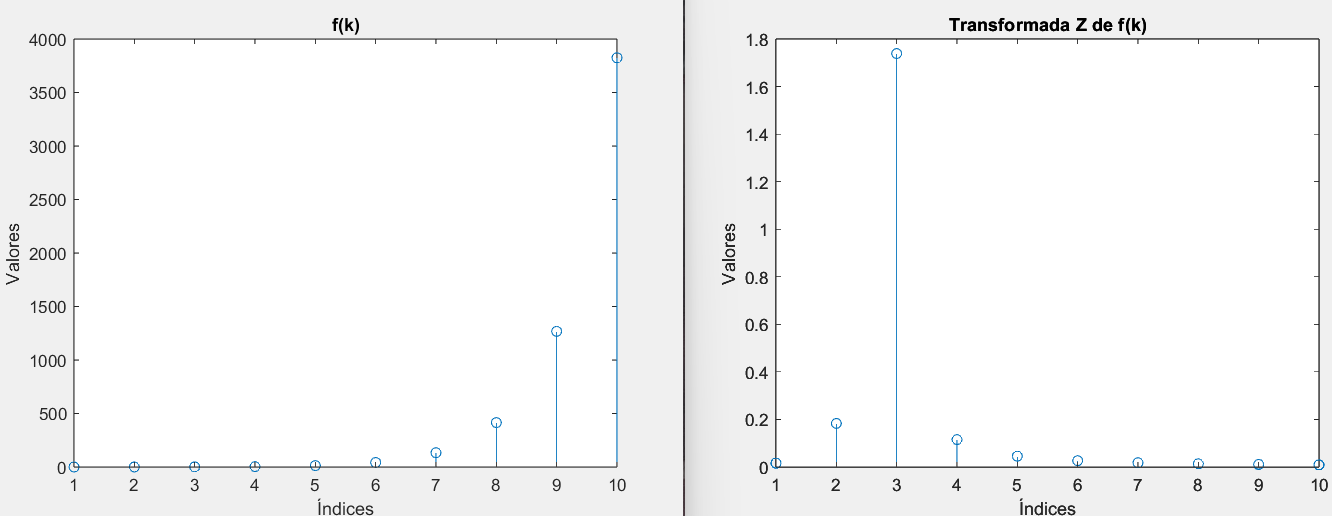
\includegraphics[width=1\textwidth]{figures/Parte2Ej1p2f2.png}
        \caption{Ejecución 2 ejercicio 1.2.}
    \end{figure}

    \newpage
    \subsection{}
    \paragraph{Dada la siguiente función de transferencia discreta:\\ \[ T(z) = \frac{0.4 \cdot z^2}{z^3 - z^2 + 0.1z + 0.02} \] \\ {\small Obtenga y represente la respuesta al impulso del sistema. \\ Obtenga y represente la respuesta del sistema ante una entrada escalón.}}

    \subsubsection*{Código}
	\inputminted[fontsize=\scriptsize, linenos, breaklines=true, xleftmargin=0.75cm, frame=lines]{matlab}{code/parte2/Ej1p3.m}

    \begin{figure}[ht]
		\begin{subfigure}{0.49\textwidth}
			\centering
			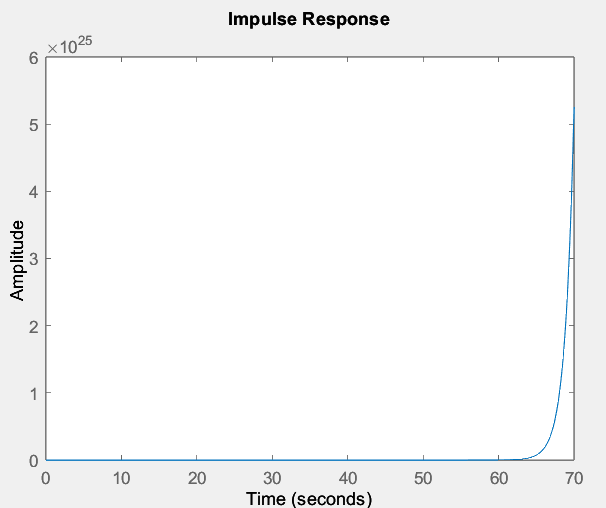
\includegraphics[width=\textwidth]{figures/Parte2Ej1p3f1.png}
            \caption{Ejecución 1 ejercicio 1.2.}
		\end{subfigure}
		\begin{subfigure}{0.49\textwidth}
			\centering
			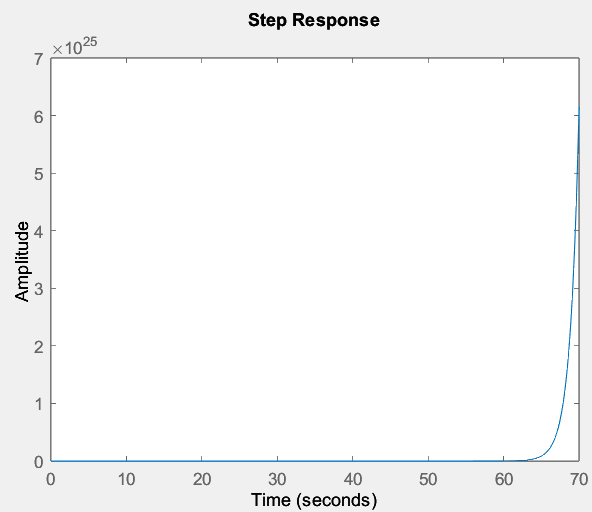
\includegraphics[width=\textwidth]{figures/Parte2Ej1p3f2.png}
            \caption{Ejecución 2 ejercicio 1.3.}
		\end{subfigure}
	\end{figure}
        
    \newpage
    
	\section{Ejercicio 2. Modelado del comportamiento de un robot móvil en Simulink.}
	
	\subsection{Implementación de las ecuaciones de movimiento siguiendo el modelo del enunciado de la práctica.}

    \begin{figure}[htp!]
	\centering
		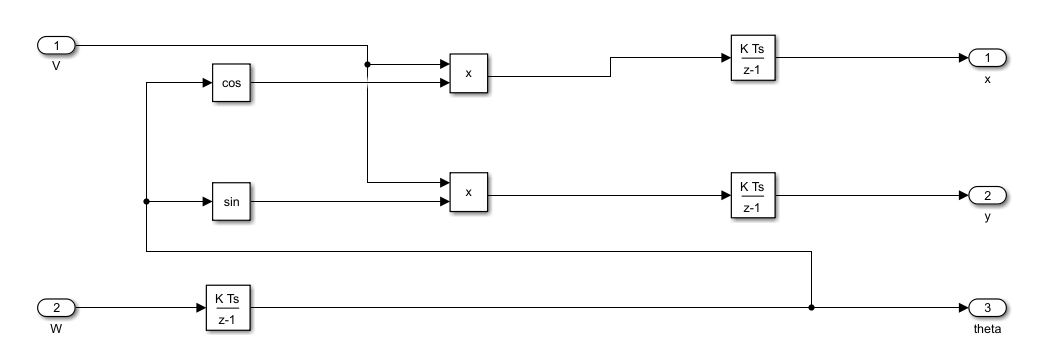
\includegraphics[width=0.6\textwidth]{figures/Parte2Ej2p1.png}
		\caption{Implementación de las ecuaciones de movimiento del robot.}
	\end{figure}

    \subsection{Montaje de la simulación del movimiento del robot.}
        
    \begin{figure}[htp!]
	\centering
		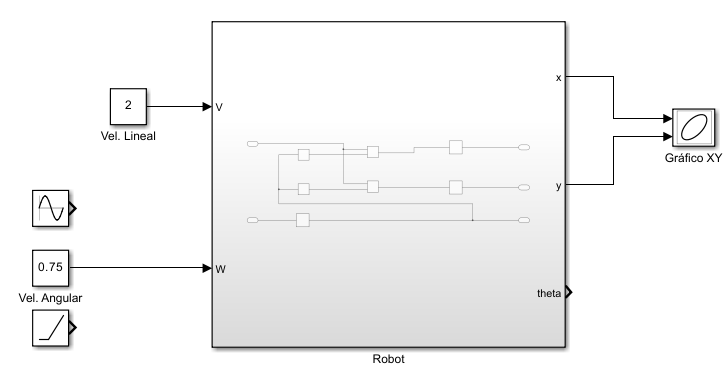
\includegraphics[width=0.7\textwidth]{figures/Parte2Ej2p2f1.png}
		\caption{Sistema robot.}
	\end{figure}
    \newpage
    \subsection{Simulación del movimiento del robot.}
    
    El movimiento del robot al tener una velocidad angular constante debería describir una circunferencia. Al hacer funcionar el sistema observamos (figura 18) la generación de una elipse, pero al fijarnos detenidamente podemos ver que el ancho y alto de la elipse son iguales y el espacio está siendo deformado automáticamente por Simulink (Cada cuadrado de la cuadrícula tiene un ancho de 0.2 y un alto de 0.5). En conclusión, el comportamiento del sistema es el esperado.
        
    \begin{figure}[htp!]
	\centering
		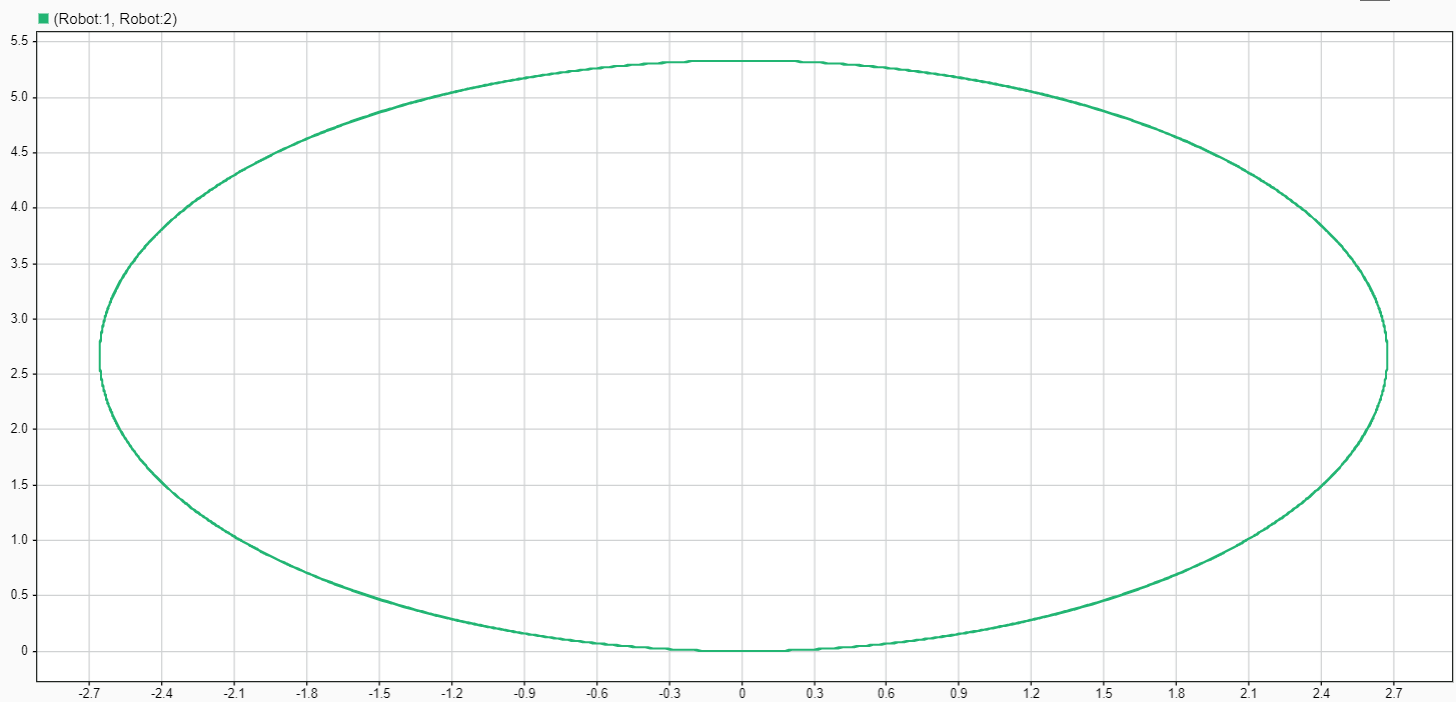
\includegraphics[width=0.7\textwidth]{figures/Movimiento_vcelocidad_constante.png}
		\caption{Movimiento del robot con Vel. Angular constante (x0.75).}
	\end{figure}

    \newpage
    \subsection{Simulación del movimiento del robot con velocidades angulares no constantes.}
        
    \subsubsection{Velocidad angular con función de rampa.}

    \begin{figure}[htp!]
	\centering
		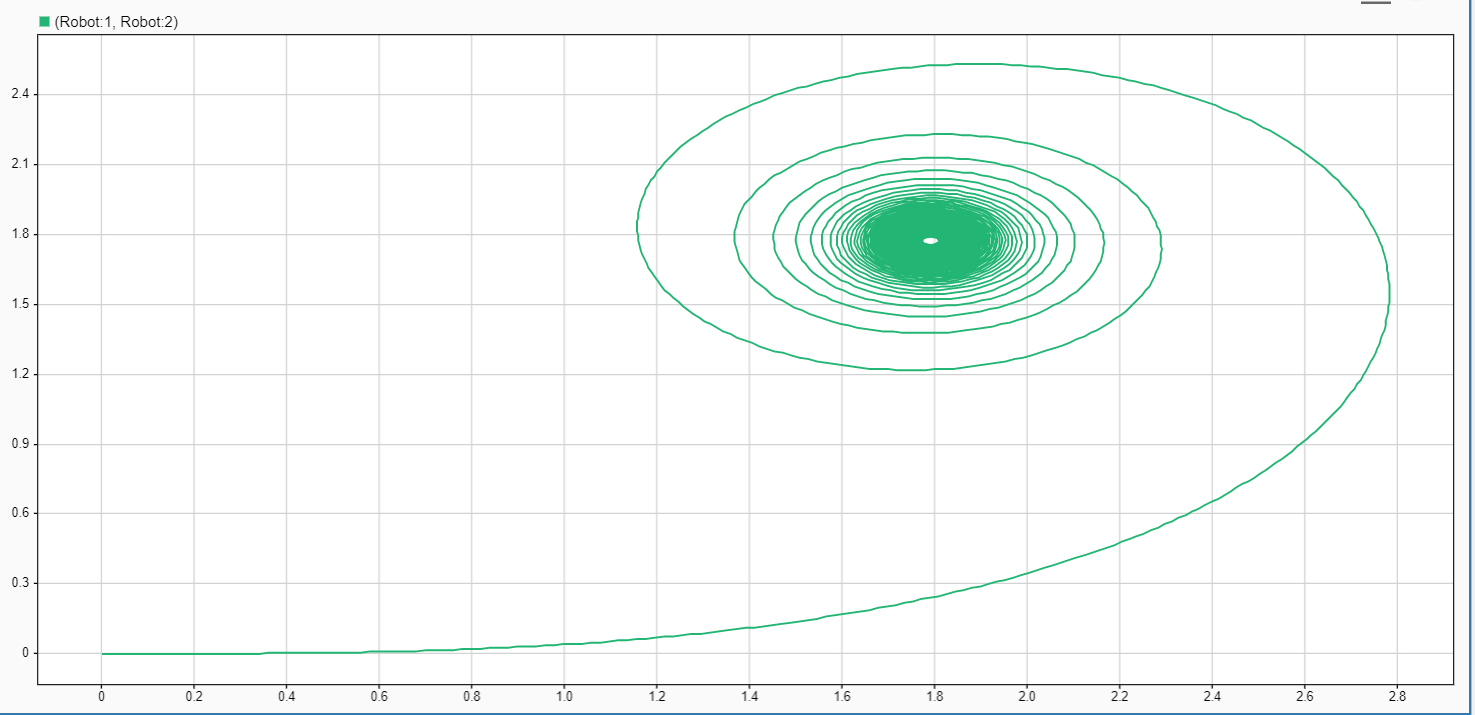
\includegraphics[width=0.7\textwidth]{figures/Movimiento_robot_rampa.png}
		\caption{Movimiento del robot con Vel. Angular con función rampa.}
	\end{figure}

    Dado que la función de rampa en Simulink es creciente, esta hace que la velocidad angular del robot aumente constantemente, resultando en que la posición del robot converja gradualmente hacia un punto específico. Podemos observar que el sistema exhibe el comportamiento esperado.

    \subsubsection{Velocidad angular con función sinusoidal.}

        \begin{figure}[htp!]
		\centering
		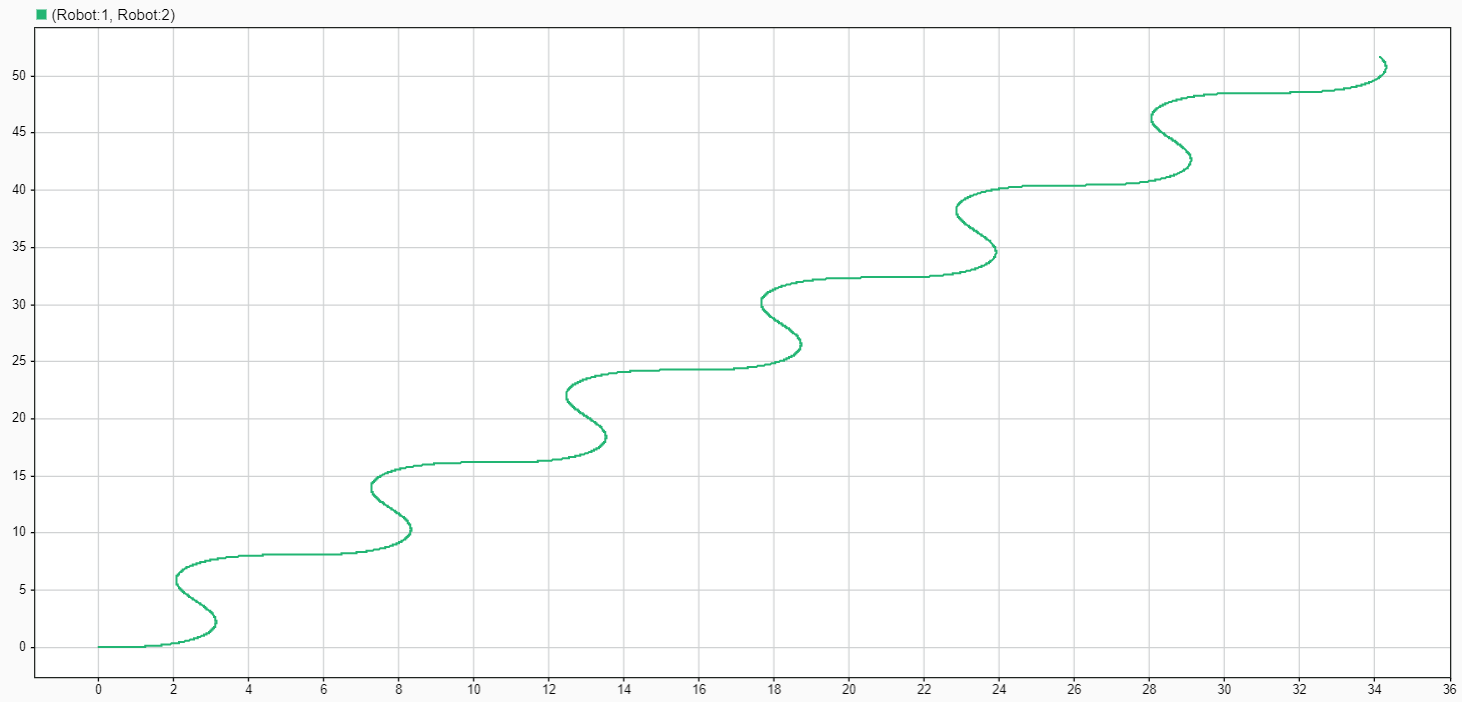
\includegraphics[width=0.7\textwidth]{figures/Movimiento_robot_sinusoidal.png}
		\caption{Movimiento del robot con Vel. Angular con función sinusoidal.}
	\end{figure}
        Podemos observar que el movimiento del robot es similar a una función trigonométrica (sen/cos), aplanada automáticamente por el programa y claramente siguiendo una trayectoria diagonal. Esta trayectoria diagonal probablemente se deba a la velocidad y posiciones iniciales del robot.

    \subsection{Simulación del movimiento del robot partiendo de la posición (-4, -4).}

    Para alterar la posición inicial del robot, se ha realizado una modificación en el sistema, añadiendo 4 bloques "Decrement Real World" a las variables de salida x e y.

    \begin{figure}[htp!]
	\centering
		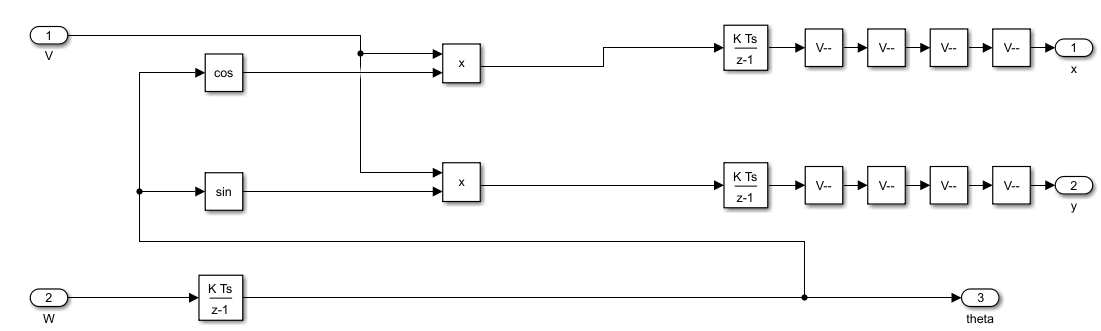
\includegraphics[width=0.7\textwidth]{figures/SistemaPosicionCambiada.png}
		\caption{Movimiento del robot con Vel. Angular con función sinusoidal.}
	\end{figure}

    \begin{figure}[ht]
		\begin{subfigure}{0.49\textwidth}
			\centering
			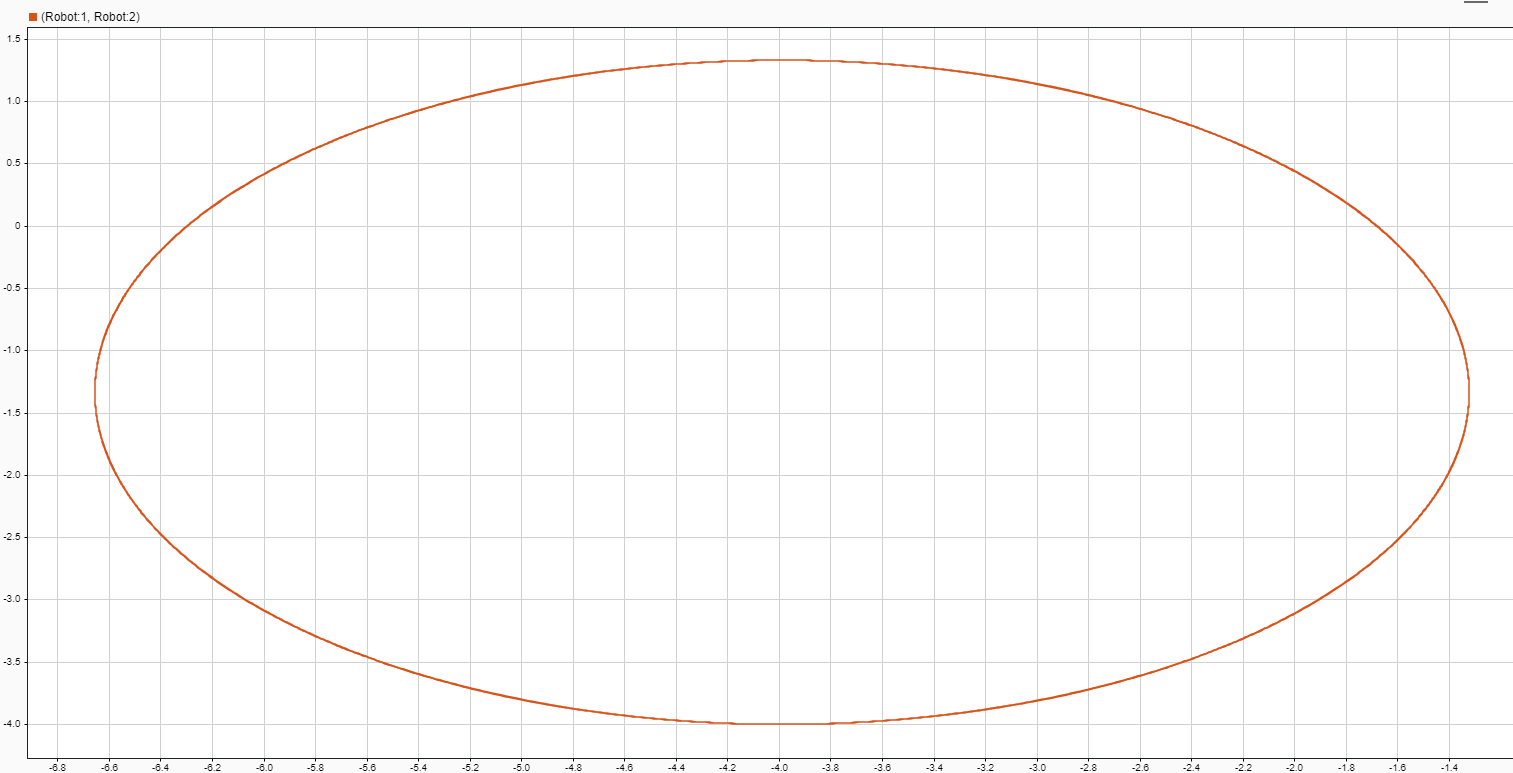
\includegraphics[width=\textwidth]{figures/Velocidad_Angular_Constante_pos_cambiada.png}
			\caption{Movimiento del robot con Vel. Angular constante (x0.75) empezando en (-4, -4)}
		\end{subfigure}
		\begin{subfigure}{0.49\textwidth}
			\centering
			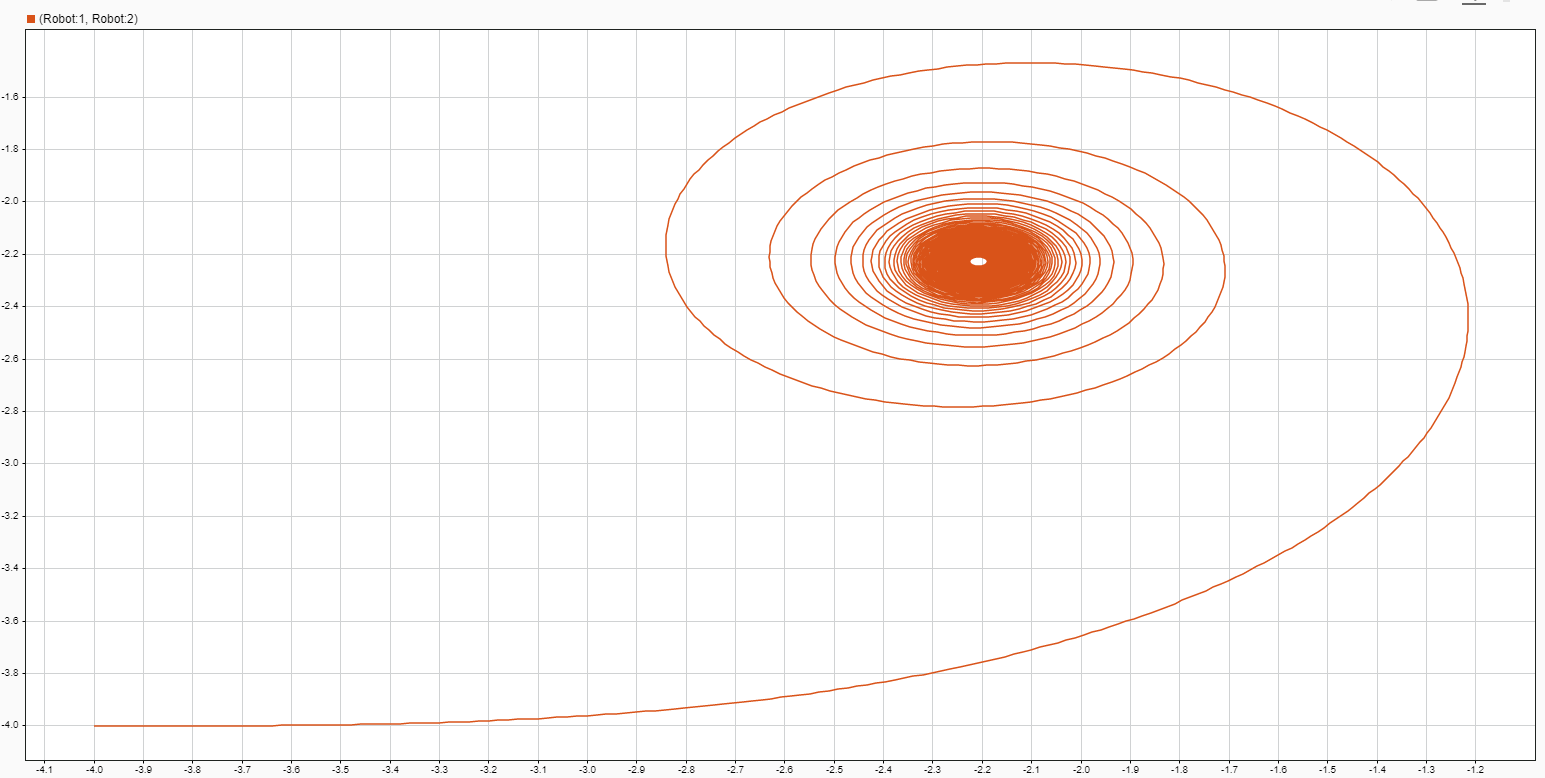
\includegraphics[width=\textwidth]{figures/VA_rampa_pos_cambiada.png}
			\caption{Movimiento del robot con Vel. Angular con función rampa empezando en (-4, -4)}
		\end{subfigure}
		\begin{subfigure}{0.49\textwidth}
			\centering
			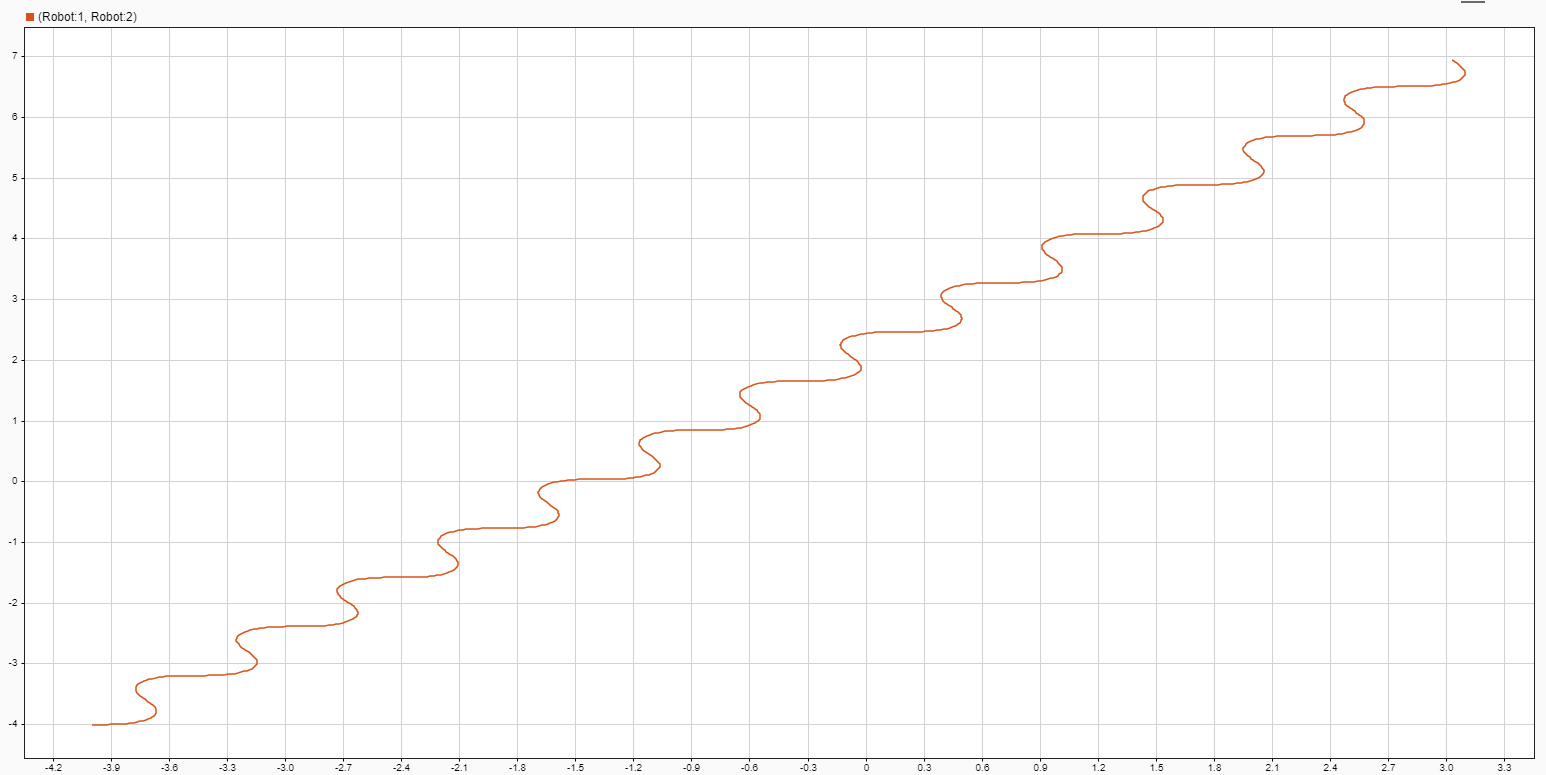
\includegraphics[width=\textwidth]{figures/VA_sin_pos_cambiada.png}
			\caption{Movimiento del robot con Vel. Angular con función sinusoidal empezando en (-4, -4)}
		\end{subfigure}
	\end{figure}

        Las gráficas tienen la misma forma, con cada punto a desplazado 4 unidades hacia abajo y hacia la izquierda
\end{document}